\documentclass[12pt,a4paper]{article}
\usepackage[utf8]{inputenc}
\usepackage{amsmath}
\usepackage{amsfonts}
\usepackage{amssymb}

\usepackage{listings}

\usepackage{multirow}

\usepackage{graphicx}
\usepackage{epstopdf} % for eps file

\usepackage{fullpage} % utilize paper space :)

\usepackage{float} % for use of [H] in figure alignment
\usepackage{subcaption} % for use of [H] in figure alignment
\usepackage{tikz}

\setlength{\parindent}{0pt}
\setlength{\parskip}{0.5\baselineskip}%

\begin{document}

\title{Statistical Machine Learning\\Exercise 2\\{\large\emph{Group 3}}}
\author{Nikolaj Iversen and Lukas Schwartz}
\date{March 15$^{th}$, 2015}
\maketitle

\vfill
\begin{center}
\includegraphics[width=0.7\textwidth]{graphics/digit_example}
\end{center}

\newpage

\tableofcontents
\listoffigures
\listoftables

\newpage


%\section{K-Nearest Neighbours}

% % % Part one
% \subsection{K-NN Theory}
The K-Nearest Neighbour (K-NN) method is in this report used to classify a specific unknown character to a set of characters ranging from 0 to 9.
The method utilizes the euclidean distance to the nearest characters



% %\subsection{K-NN Implementation}
The K-NN algorithm is implemented as in code \ref{code:KNN_implementation}.
The implementation of how the result of the voting is calculated, is not shown here.


\lstinputlisting[language = R,
firstnumber = 291,
firstline = 291, 
lastline = 311, 
captionpos=b,
caption = {K-NN implementation.},
label = {code:KNN_implementation}]{../Code/KNN/01/test.R}


The function takes three arguments, \texttt{testVector}, \texttt{trainVectors} and \texttt{k}. 
\texttt{testVector} is a vector containing the set of pixel values of the character that is wished identified. 
\texttt{trainVectors} is a three dimensional set of vectors. 
This makes it possible to distinguish between the character represented by the group and the individual characters and their data.

Line 290 to 293, in code \ref{code:KNN_implementation}, defines the two arrays \texttt{neighbours} and \texttt{testDistance}.
These are used to store the \texttt{k} nearest neighbours and calculate the distance between two characters respectively.

The code then, in line 295 to 299, loops through all the different character groups and the characters within.
For each character the distance is then calculated to the \texttt{testVector}.
If the distance is smaller than that of one of the previously inserted into \texttt{neighbours}, 
then lines 301 to 309 insert it into the \texttt{neighbours} list in sorted order and the one furthest away is removed.

Once this is done, the \texttt{neighbours} list can then be inspected to guess which character it is.

% \subsection{Person Dependent}
This section tests the KNN algorithm explained earlier using data from one single person, namely Group three member two's data.
The test are performed first with the data split equally into a 50\% for the training and 50\% for the test set.
Afterwards with a 90/10\% split for training and test respectively is computed.
Both test where conducted using cross validation with 10 runs.

\subsubsection{Equally Sized training and test set}
Figure \ref{fig:PersonDependentPerformance_5050} shows a test with 50/50\% split was carried out for changing \textit{K}'s.

\begin{figure}[H]
\centering
% figure...
\caption{Test result with a 50/50\% split of group three member two's data with changing values for \textit{K}. The data points are taken as the mean of 10 runs using cross validation.}
\label{fig:PersonDependentPerformance_5050}
\end{figure}

As seen on figure \ref{fig:PersonDependentPerformance_5050} then \textbf{...}.


\subsubsection{90/10 Data Split}
A cross validation was also carried out using a 90/10\% split of the data. 
The result of this is seen in figure \ref{fig:PersonDependentPerformance_9010}.


\begin{figure}[H]
\centering
% figure...
\caption{Test result with a 90/10\% split of group three member two's data with changing values for \textit{K}. The data points are taken as the mean of 10 runs using cross validation.}
\label{fig:PersonDependentPerformance_9010}
\end{figure}

Figure \ref{fig:PersonDependentPerformance_9010} \textbf{...}.



% % 1.6.2: tabel over mean+var over 10 runs + 
%        graf dpi vs success for filtre (10 run)

\subsection{Preprocessed Image - Single Person Tests}

\begin{table}[h]
\centering
    \begin{subtable}[b]{0.56\textwidth}
    \centering
        \begin{tabular}{lcccccc}
            &Raw	& Avg	& G 0.5	& G 1	& G 2 \\
\hline
100	& 0.8297	& 0.8297	& 0.8788	& 0.8545	& 0.7750 \\
200	& 0.8635	& 0.8635	& 0.9180	& 0.8998	& 0.8602 \\
300	& 0.8925	& 0.8925	& 0.9373	& 0.9190	& 0.8842 \\

        \end{tabular}
        \caption{Mean success rate.}
    \end{subtable}
    \begin{subtable}[b]{0.56\textwidth}
    \centering
        \begin{tabular}{lcccccc}
            &Raw	& Avg	& G 0.5	& G 1	& G 2 \\
\hline
100	& 0.83	& 0.83	& 0.86	& 0.85	& 0.78 \\
200	& 0.86	& 0.86	& 0.90	& 0.90	& 0.86 \\
300	& 0.89	& 0.89	& 0.92	& 0.92	& 0.88 \\

        \end{tabular}
        \caption{Variance in success rate.}
    \end{subtable}
    \caption[Success of smoothing functions.]{Mean success rate and variance of different smoothing functions.}
    \label{tb:smooth}
\end{table}

\begin{figure}[h]
\centering
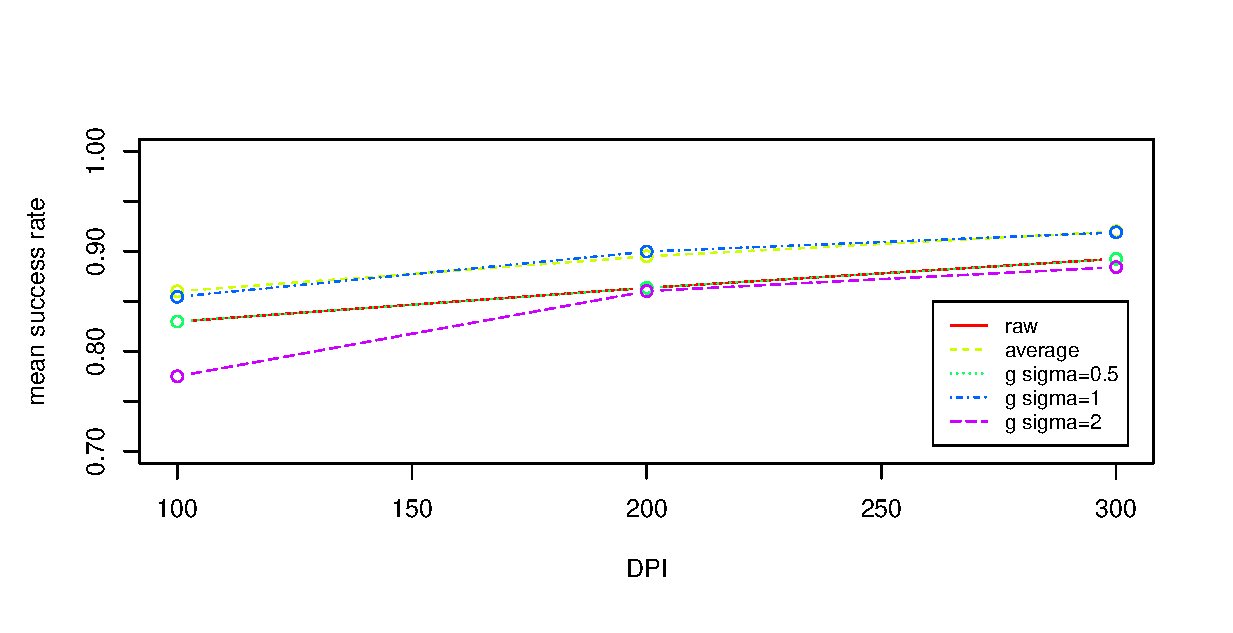
\includegraphics[width=1\textwidth]{graphics/smoothing}
\caption{Success rate of smoothing functions.}
\label{fig:smooth}
\end{figure}

Applying a smoothing function can give the image an advantage when using the nearest neighbour analysis.
By taking an average of the neighbouring pixels the lines in the digit should be wider and the digits should have a better chance of overlapping.
The danger is that too much smoothing could make the whole image one colour and would completely destroy any chance of analysis.
A Gaussian distribution (also referred to as a normal distribution) a naturally occurring distribution that happens when a random result occurs around a mean. 
The $\sigma$ signifies the deviation of the distribution. 
The 2D equation of a Gaussian distribution is shown in equation \ref{eq:gauss}. 

\begin{equation}
G(x,y) = \frac{1}{2\pi \sigma^2} e^{- \frac{x^2+y^2}{2\sigma^2}} \label{eq:gauss}
\end{equation}

Using the Gaussian filter to smooth an image will weigh the distance to the pixel.
A small $\sigma$ will make a small deviation and thus heavily weigh the center pixel.
The results of the filtering methods were also compared to the raw image with 100, 200 and 300 DPI.
These results are compared with an averaging filter (avg) which takes the average of the four neighbouring pixels and a Gaussian filter (G) with different values for sigma.
These tests were done 10 times, using cross validation, and the mean of each success rate is plotted in figure \ref{fig:smooth}. 
Since the variance is too small to be seen in the figure the mean and variance is shown in table \ref{tb:smooth}.
The averaging filter does not give a measurable different result from not using a filter.
The Gaussian filter does improves the success rate for some values of sigma, but a larger $\sigma$ makes it worse.


%\section{K-NN on Big Data}
%\section{Introduction}

The classification of handwritten characters is used in a wide range of products to day.
Hence, this report goes in depth with how the numbers from zero to nine can be classified using machine learning algorithms.

The data set consists of a set of handwritten characters from zero to nine.
These were constructed by the students enrolled in the course Statistical Machine learning (RM-SML-E1) in 2015 at the University of Southern Denmark (SDU).
The characters were written in boxes of $0.55 \times 0.55 \textit{ cm}$ on a sheet with $20 \times 20$ boxes for each character.
The set used in this report is the 100DPI dataset.
Each number is hence stored as a $20 \times 20 \textit{ pixel}$ matrix containing the handwritten character.

The methods used for classification are K-Nearest Neighbours and Decision Trees.
This is to compare a method of lazy supervised learning against a method of supervised learning.
Furthermore a set of different ways to pre-process the data is explored.
Finally the two methods are compared with each at the best parameters and preprocessing settings.

The goal is to tests the handwritten digits from 20 people enrolled in the course.
The first test is where all people are mixed together, everybody contributing 90\% of their data to the training set and 10\% to the test set.
This is considered the easy problem as special ways of writing a digit will be represented in the training data.

Another test is to use 19 people's digits as training data and use the last person to test.
This is considered the hard problem.

To test the performance of the classification methods a simplified problem has been constructed.
It takes training data from a single person, Lukas Schwartz, which is referred to as Group 3 member 2 (G3M2).
By splitting the data 90\% for training and 10\% for testing
360 digits from each class as training data and 40 digits was used.
Testing each parameter with the simplified problem means the parameters could be tested in less time than if using the entire data set.

%% % Part two
%\subsection{K-NN on Big Data}
The K-NN algorithm can be seen to be approximately linear on figure \ref{fig:predictionTimeVStrainSize}.
It takes approximately 0.47 seconds to predict a single value.

\begin{figure}[H]
\centering
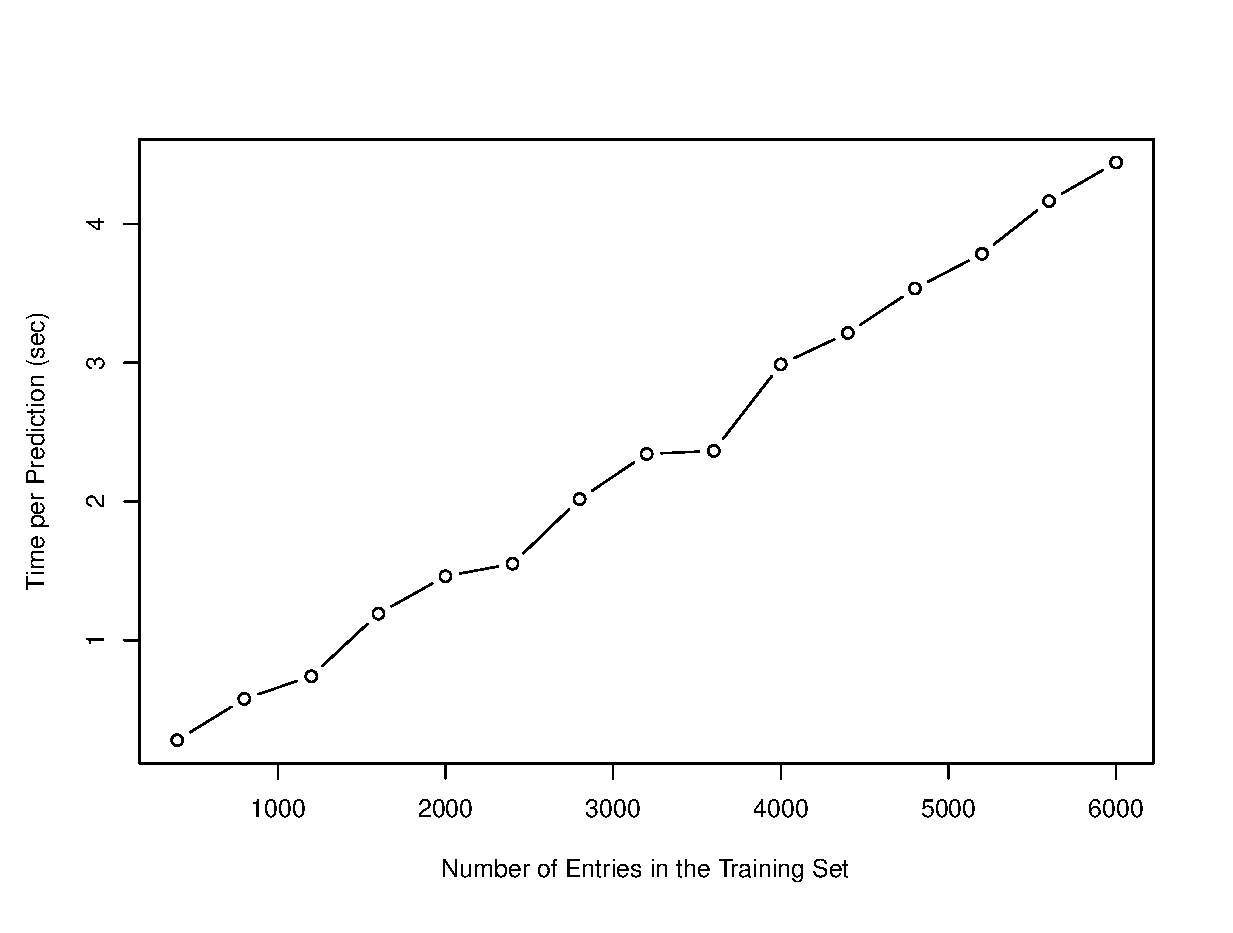
\includegraphics[width = 0.95 \textwidth]{graphics/graph_timeVSppl}
\caption{The time taken for one prediction for different training set sizes at 100 DPI resolution.}
\label{fig:predictionTimeVStrainSize}
\end{figure}

This can, when a lot of values, such as the 4000 elements dataset of a single person, take a long time to predict all of them (approx. 30 min on 100 DPI).
It is therefore desirable to bring down the prediction time.
This will be considered in the following chapters.

%
%\subsection{Principle Component Analysis}


\begin{figure}[H]
\centering
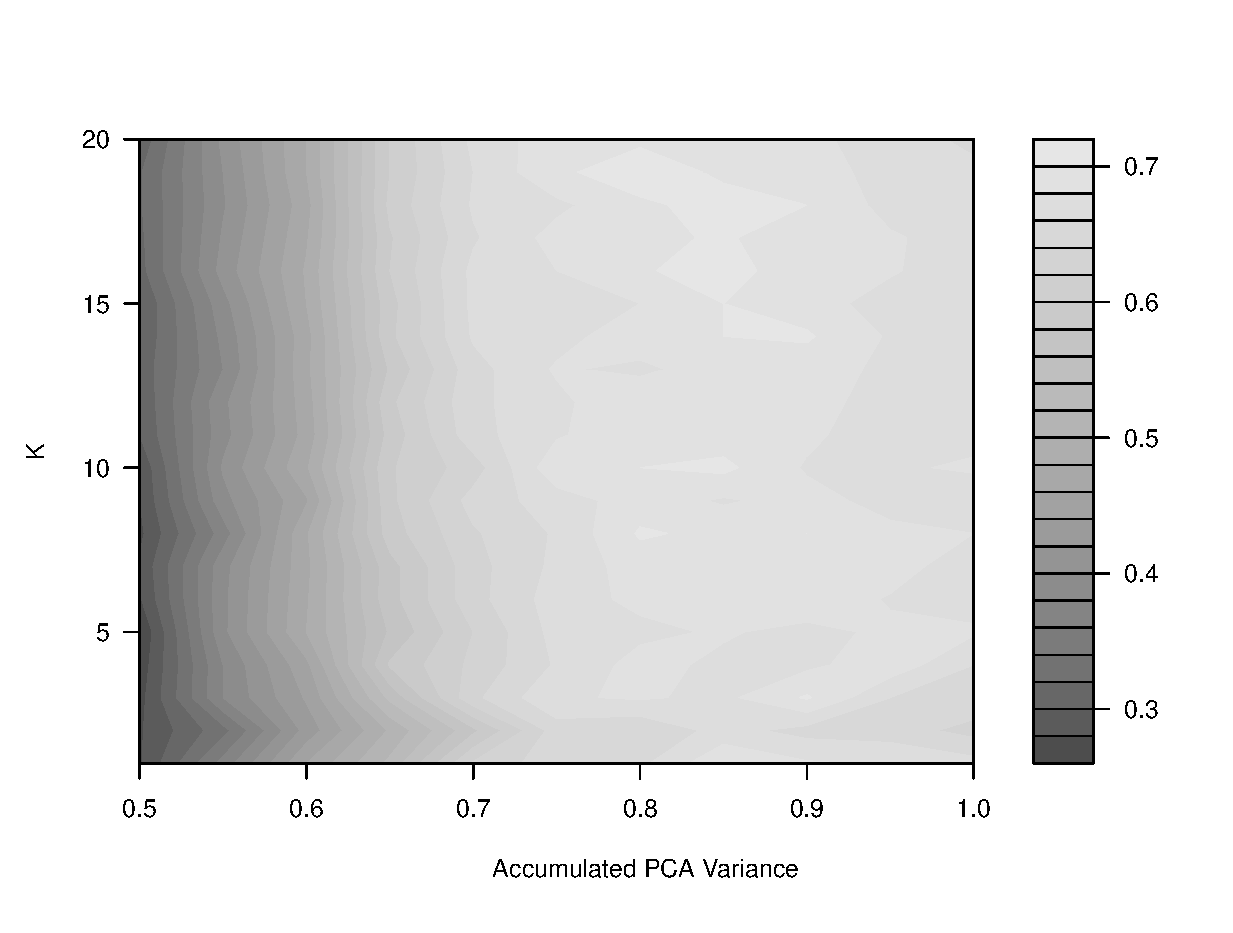
\includegraphics[width = 16cm]{graphics/contour_k_PCA_oneVsRest}
\caption{Success rate for detection of characters of Group 3 Member 2's data when he himself is not represented in the training set. 
Thewas tested with 16 people.}
\label{fig:}
\end{figure}


\begin{figure}
\centering
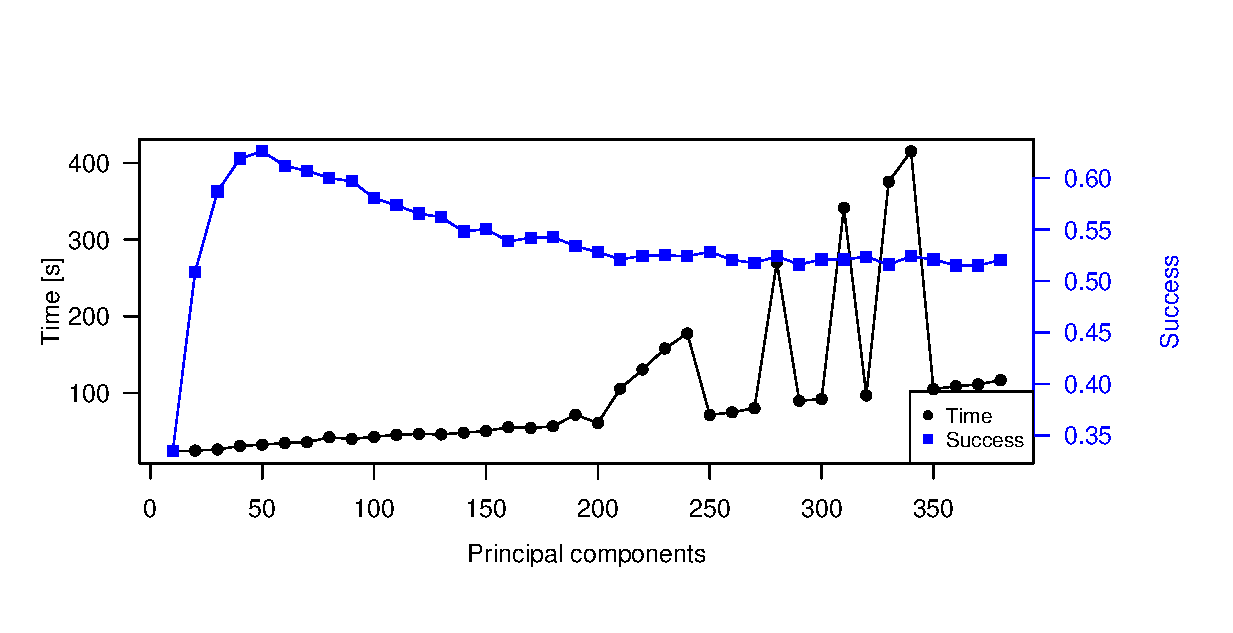
\includegraphics[width =0.8 \textwidth]{graphics/pca_timing}
\caption{Timing of running the PCA with different principle components. 
The data was run on Group 3 member 1's data on 100 DPI. 
The percentage of successful predictions is also measured with the same data.}
\label{fig:pca_timing}
\end{figure}

\begin{figure}
\centering
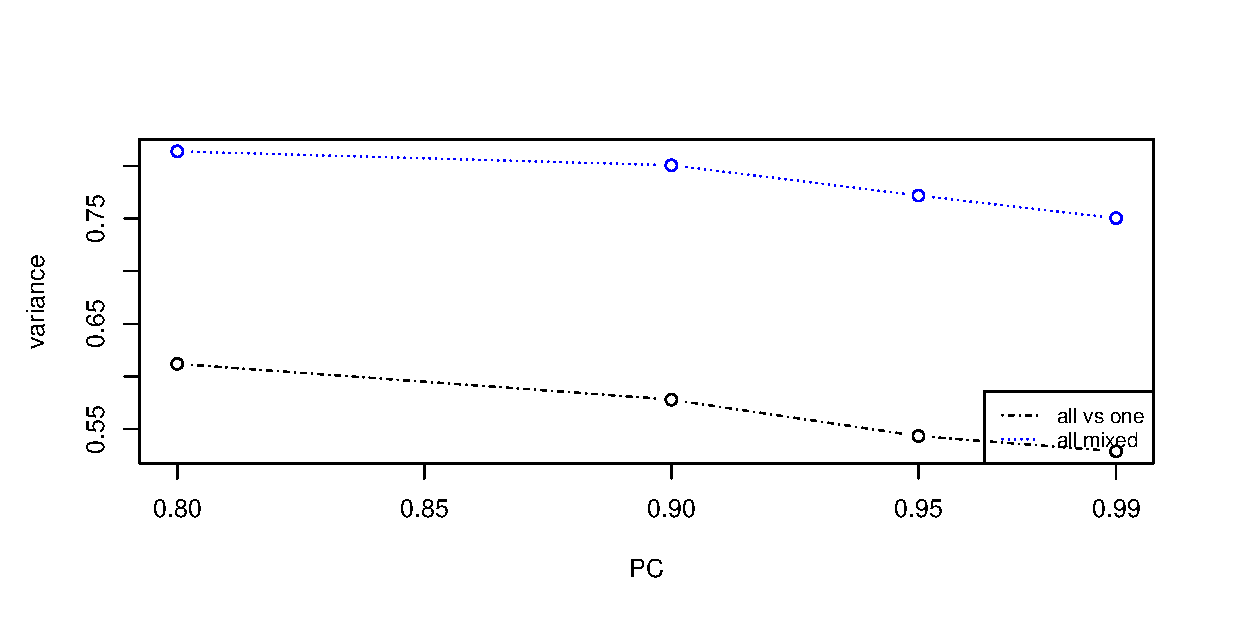
\includegraphics[width =0.8 \textwidth]{graphics/pca_success}
\caption{Percentage of successful predictions with increasing percentage of principle components used.
The data was run on Group 3 member 1's data on 100 DPI. }
\label{fig:pca_success}
\end{figure}


%
%\subsection{Data Normalization}
\label{sec:DataNormalization}
When comparing multiple entries in a dataset, it might be beneficial to normalize such to obtain a basis for equal comparison.
In the case of numbers being written and detected, such as ours, there might be differences in the colors of the characters when different pens/pencils are used.
This can create unwanted differences between elements in a category, which are else identically, and hence lead to false predictions.
Two normalization algorithms where hence implemented.
These are, min-max normalization and z-score standardization.

Figure \ref{fig:normalization_test_pre-post} shows the result when cross validation is carried out on the data from the 16 people in the class.
In figure \ref{fig:normalization_test_pre-post}, each individual is tested up against the rest of the group without contributing to the training set themselves. 
The two types of normalization are performed both before and after the data reduction using PCA.


\begin{figure}[H]
\centering
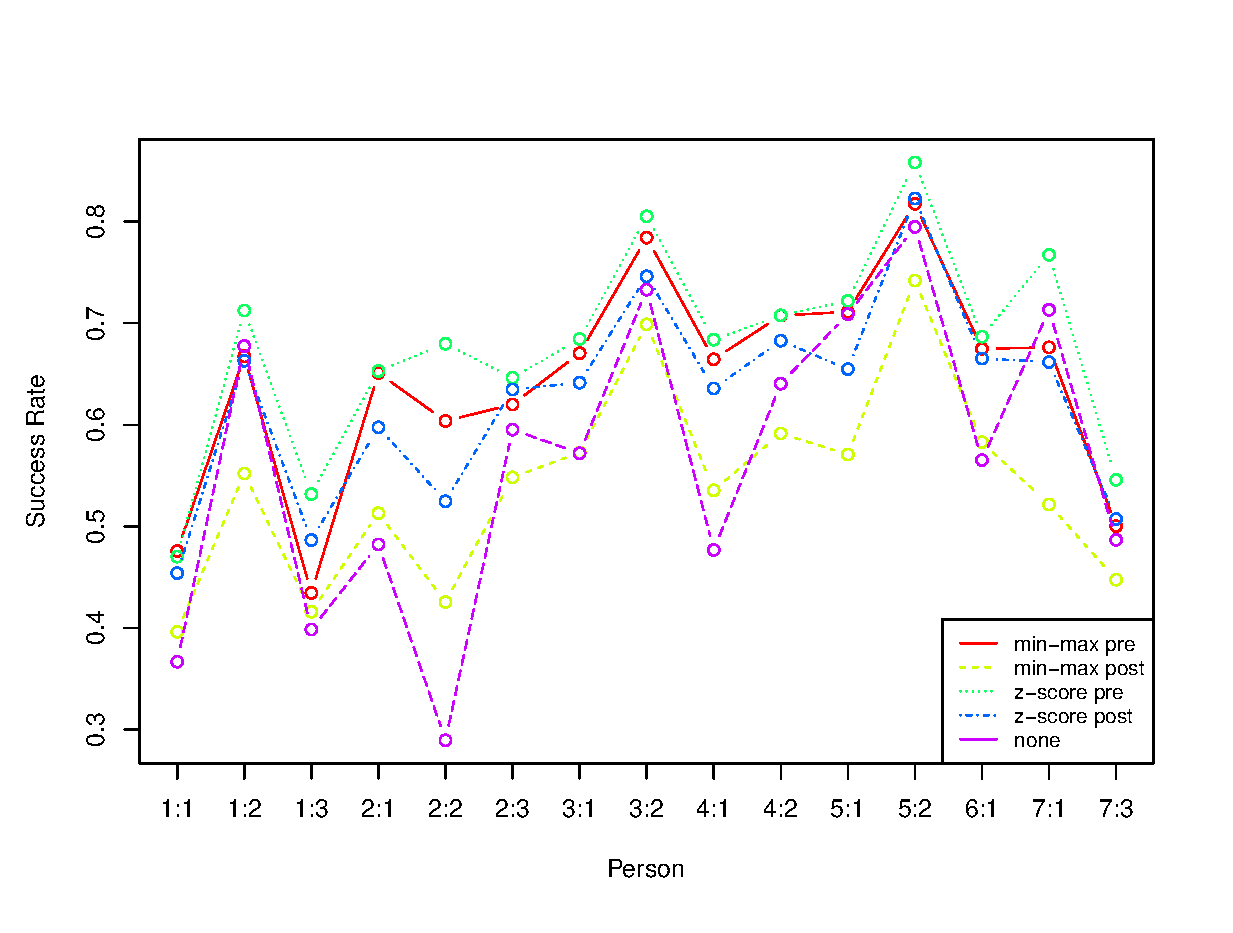
\includegraphics[width = \textwidth]{graphics/graph_normalization}
\caption[Comparison of different students.]{Success rate for detection of characters of on person when not in the training set. 
Data normalized before (pre) and after (post) dataset reduction using PCA.
PCA was set to ensure that 80\% of all variance was included in the data set and K as 10.
The person tested for is given as 'Group':'Member'.
It was tested with 16 people.}
\label{fig:normalization_test_pre-post}
\end{figure}

The mean success rate of figure \ref{fig:normalization_test_pre-post} is listed in table \ref{tab:meanSuccess_normalization_test_pre-post}.
From both the graph and table, it can be concluded that the z-score standardization before the PCA reduction performs, on average, at least 3\% better than the other methods.

The figure \ref{fig:normalization_test_pre-post} also shows that in general all three normalizations, except for the min-max normalization after PCA reduction, is on average, yielding a higher number of correct predictions.

The normalization before the PCA reductions yields a better result in all cases. 
This may be because it enables the PCA to find the features being more responsible for the decision of which category a element belongs to. 
Some of the performance improvement can be because of features of a low variance in their measured value, have a larger relevance as to what the actual category of the elements are.

\textbf{UPDATE TABLE!}

\begin{table}[H]
\centering
\begin{tabular}{|l|r|}\hline
% 0.5720167 0.4639500 0.6055167 0.5521333 0.5034333
Normalization Method & Mean Success \\ \hline
Min-Max Normalization Pre & 57.2 \% \\ \hline
Min-Max Normalization Post & 46.4 \% \\ \hline
Z-Score Normalization Pre & 60.6 \% \\ \hline
Z-Score Normalization Post & 55.2  \% \\ \hline
No Normalization & 50.3 \% \\ \hline
\end{tabular}
\caption{Mean success rates for normalization test as seen in figure \ref{fig:normalization_test_pre-post}.}
\label{tab:meanSuccess_normalization_test_pre-post}
\end{table}



\subsubsection{Performance Effect when adding a Filter}

\begin{figure}[H]
\centering
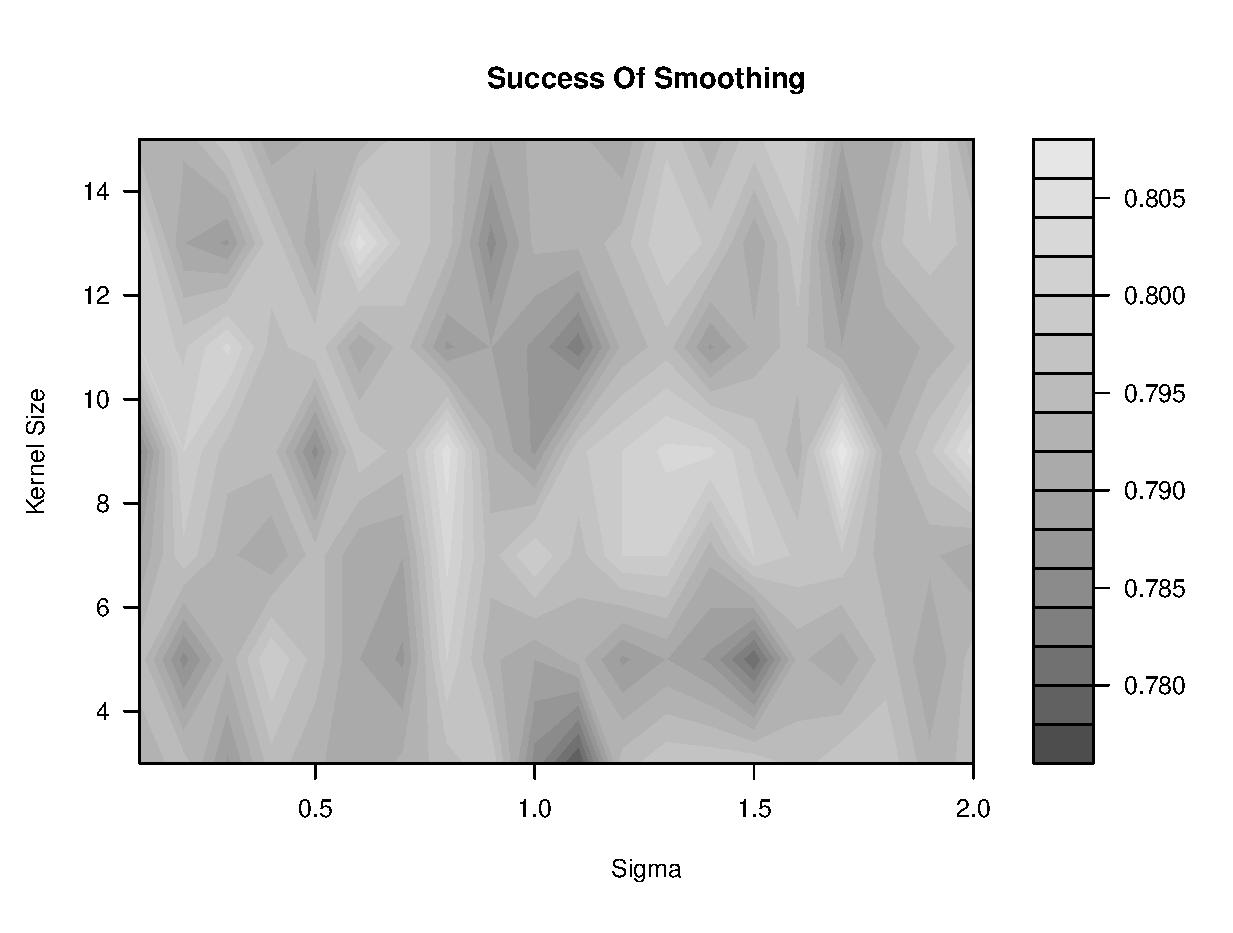
\includegraphics[width = \textwidth]{graphics/success_of_smoothing_contour}
\caption[Optimal smoothing]{Impact of sigma and kernel size when smoothing an image. 
Tested with group 3 member 2's data against 14 other students.
}
\label{fig:smoothing_contour}
\end{figure}

To find the optimal kernel size the success detection rate was plotted with a varying $\sigma$. 
The optimal kernel size is chosen to be 9 pixels wide.
From figure \ref{fig:smoothing_contour} it is concluded that a filter size of 9 is optimal.

Using this knowledge figure \ref{fig:normalization_test_with_smooth} was generated.
The figure compares the unprocessed success rate compared to that of the z-score pre and z-score pre with gaussian smoothing (filter size 9 and sigma 0.7).

 \begin{figure}[H]
 \centering
 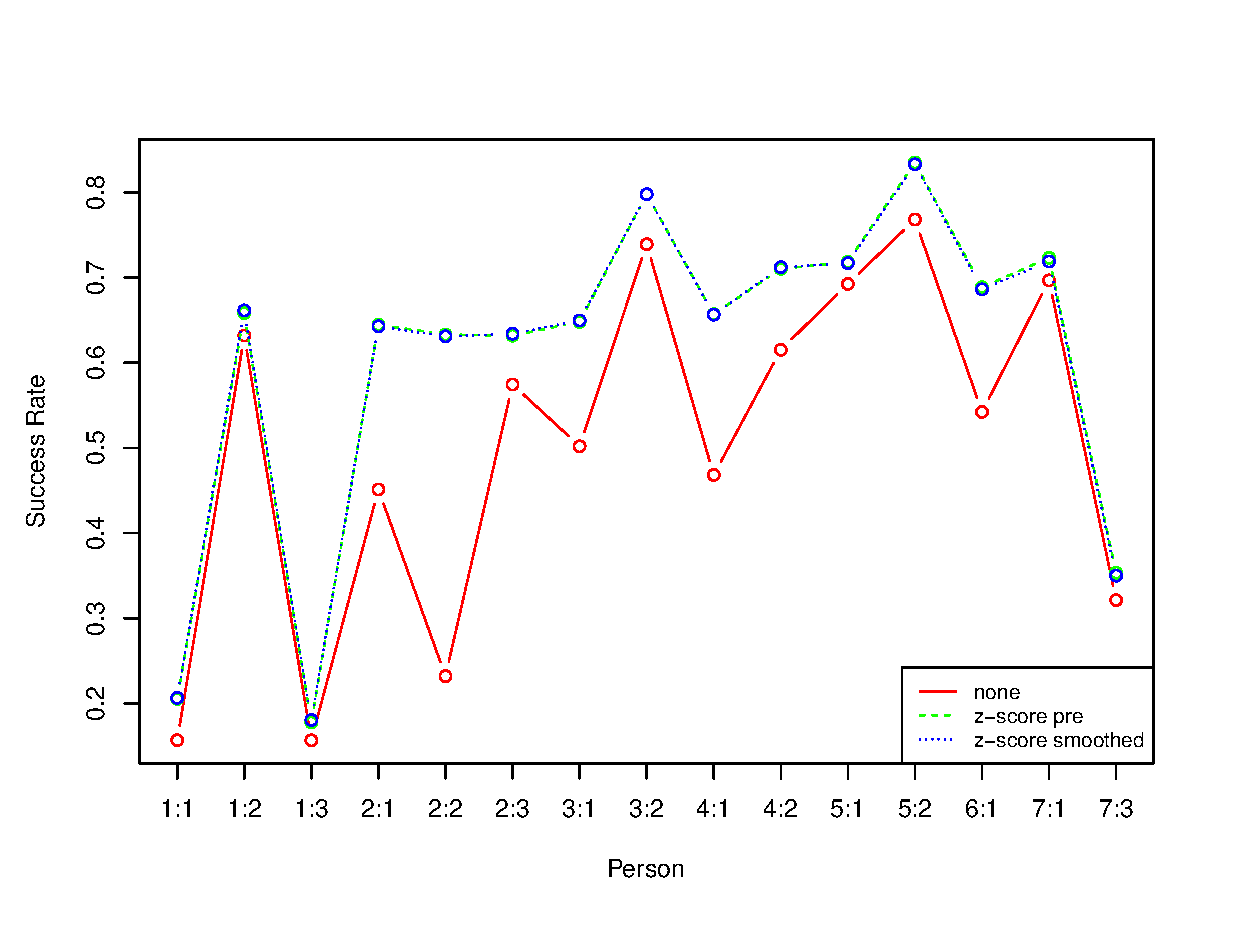
\includegraphics[width = \textwidth]{graphics/graph_normalization_smoothed}
 \caption[Filtered and normalized data.]{Filtered data normalized vs unfiltered normalized data.
 Running each person against the rest of the class in the train set.
 }
 \label{fig:normalization_test_with_smooth}
 \end{figure}

As seen on figure \ref{fig:normalization_test_with_smooth}, then the result of smoothing the data before normalization is not improving the data.

%
%\subsection{K-means}
K-means is used to group the dataset into categories depending on their location in the x-dimensional space determined by the amount of features representing one of them.
The center of these clusters are then computed and identified as a specific category.
Using these centres, a unknown element can then be categorized depending on which cluster is the closest.

To find the number of clusters best representing the dataset, then the within-group heterogeneity and homogeneity was computed for various K's as seen on figure \textbf{ref!!}.
The elbow point can from here be determined to be at \textbf{K = something}.

\begin{figure}
\centering
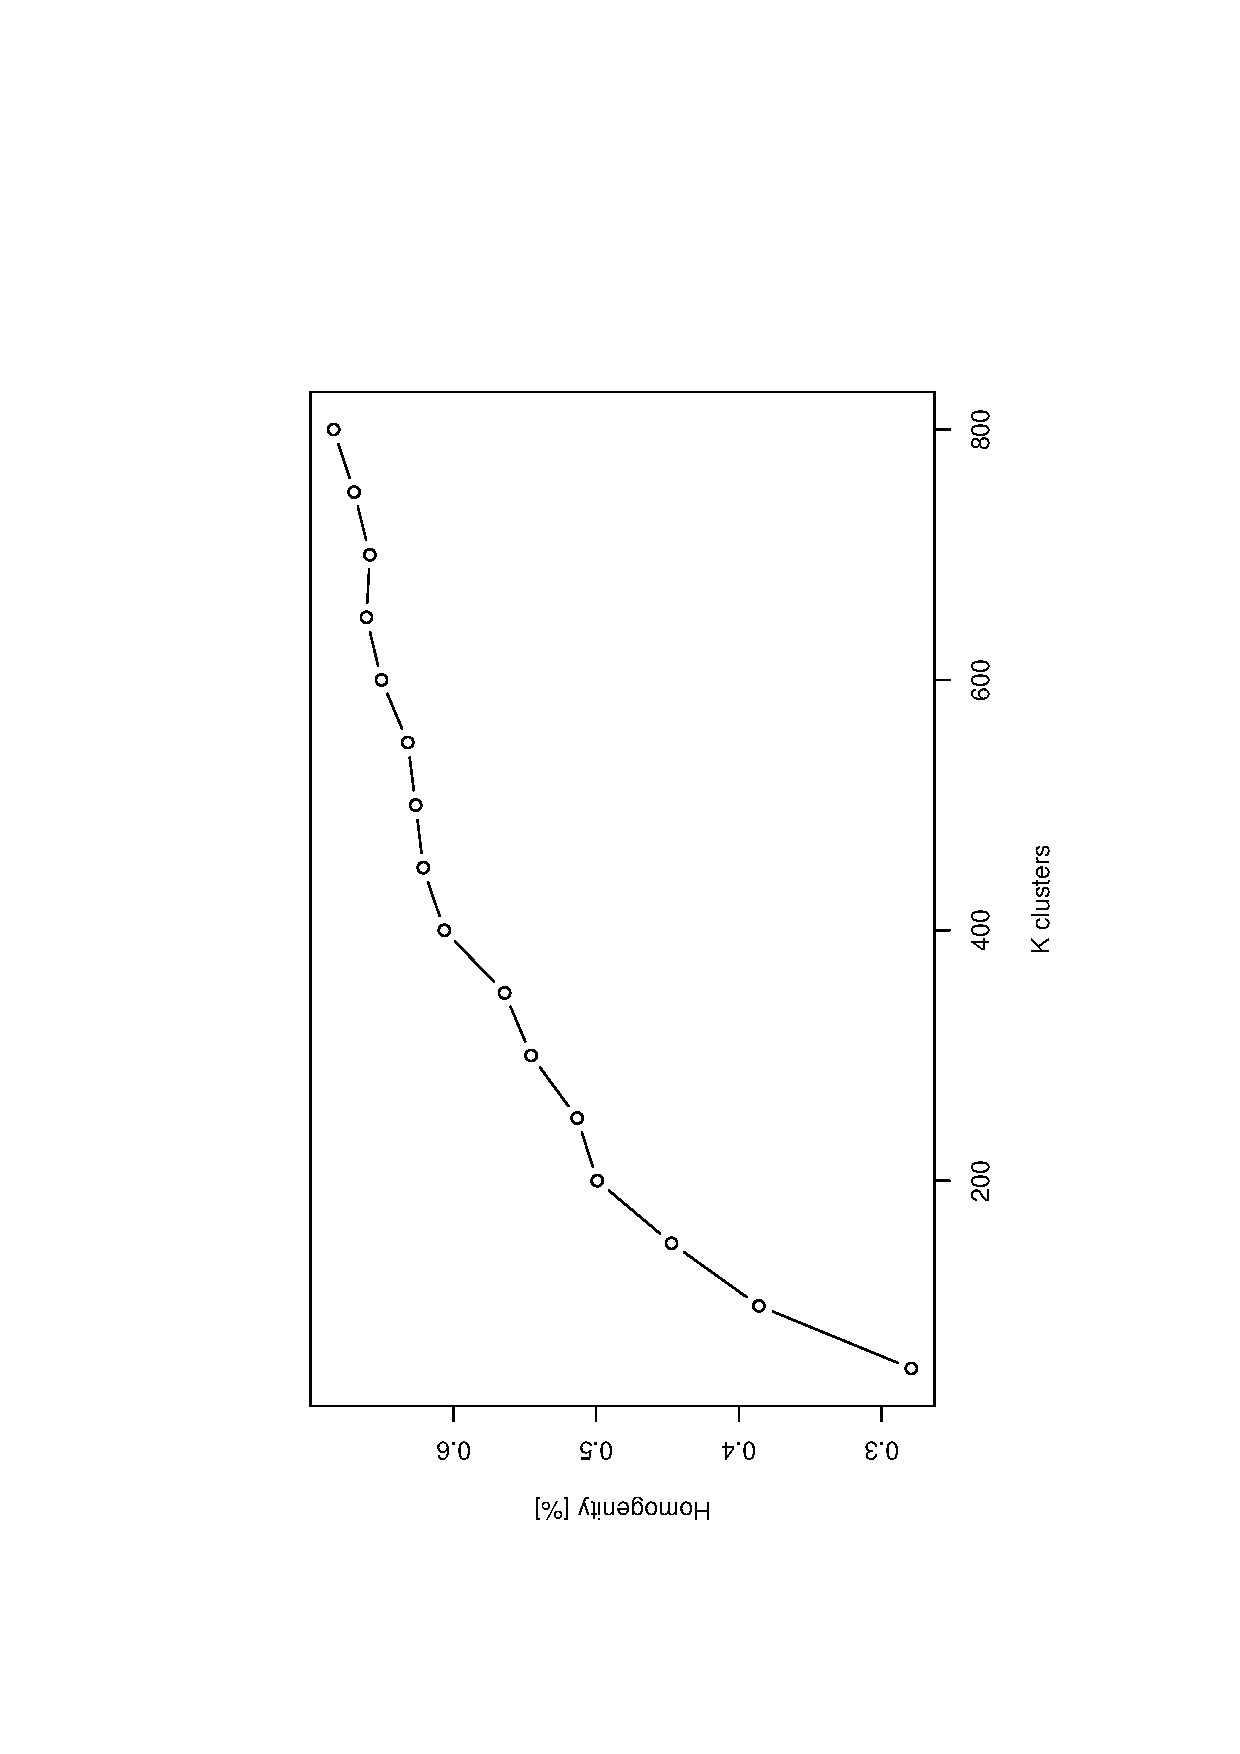
\includegraphics[width=\textwidth]{graphics/homogenity}
\caption{Homogeneity of the data set.}
\label{fig:homogeneity_kmean}
\end{figure}


\begin{figure}
\centering
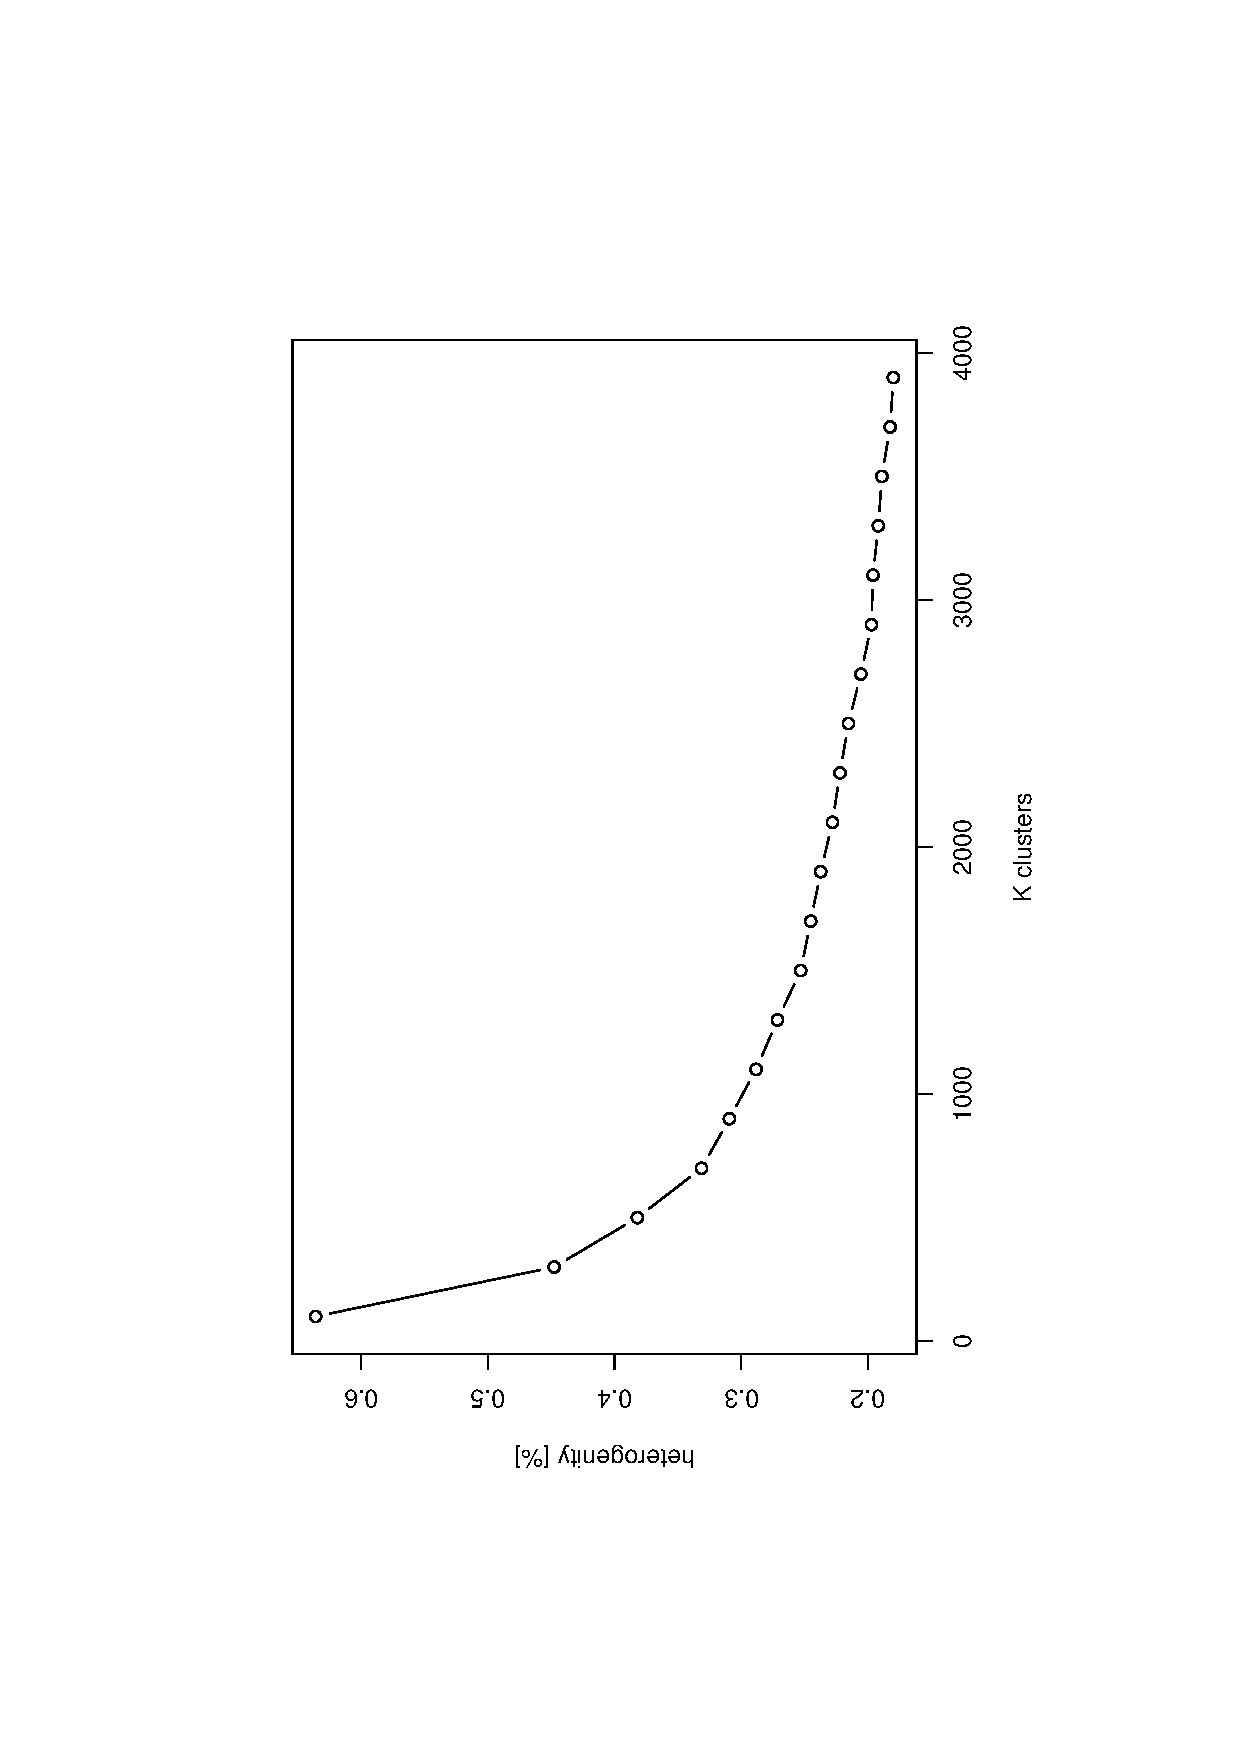
\includegraphics[width=\textwidth]{graphics/heterogenity}
\caption{Heterogeneity of the data set.}
\label{fig:heterogeneity_kmean}
\end{figure}

\begin{table}[H]
\centering
%# kmean = 400
%# k_knn = 10
%# k_mean = 10
%# kmean_iterations = 500
%# Time taken to prep kmean: 272.61"
%# [1] "Time taken to run kmean classification: 8.47000000000003"
%# [1] "Success for kmean: 0.4415"
%# [1] "Time taken to run raw knn classification: 1857.24"
%# [1] "Success for raw knn: 0.739"
\begin{tabular}{|l|r|r|}\hline
Criteria & Raw KNN & K-mean K-NN \\ \hline
Pre-Processing Time & 0s & 4m32.61s \\ \hline
Classification Time & 30m57.24s & 8.47s \\ \hline
Success Rate & 73.9\% & 44.2\% \\ \hline
\end{tabular}
\caption{Processing time comparison of running K-NN on K-mean data and raw}
\label{tab:processingtime_kmean_vs_raw_knn}
\end{table}

\section{Naive Bayes}
\section{Introduction}

The classification of handwritten characters is used in a wide range of products to day.
Hence, this report goes in depth with how the numbers from zero to nine can be classified using machine learning algorithms.

The data set consists of a set of handwritten characters from zero to nine.
These were constructed by the students enrolled in the course Statistical Machine learning (RM-SML-E1) in 2015 at the University of Southern Denmark (SDU).
The characters were written in boxes of $0.55 \times 0.55 \textit{ cm}$ on a sheet with $20 \times 20$ boxes for each character.
The set used in this report is the 100DPI dataset.
Each number is hence stored as a $20 \times 20 \textit{ pixel}$ matrix containing the handwritten character.

The methods used for classification are K-Nearest Neighbours and Decision Trees.
This is to compare a method of lazy supervised learning against a method of supervised learning.
Furthermore a set of different ways to pre-process the data is explored.
Finally the two methods are compared with each at the best parameters and preprocessing settings.

The goal is to tests the handwritten digits from 20 people enrolled in the course.
The first test is where all people are mixed together, everybody contributing 90\% of their data to the training set and 10\% to the test set.
This is considered the easy problem as special ways of writing a digit will be represented in the training data.

Another test is to use 19 people's digits as training data and use the last person to test.
This is considered the hard problem.

To test the performance of the classification methods a simplified problem has been constructed.
It takes training data from a single person, Lukas Schwartz, which is referred to as Group 3 member 2 (G3M2).
By splitting the data 90\% for training and 10\% for testing
360 digits from each class as training data and 40 digits was used.
Testing each parameter with the simplified problem means the parameters could be tested in less time than if using the entire data set.


\subsection{Data Normalization}
\label{sec:DataNormalization}
When comparing multiple entries in a dataset, it might be beneficial to normalize such to obtain a basis for equal comparison.
In the case of numbers being written and detected, such as ours, there might be differences in the colors of the characters when different pens/pencils are used.
This can create unwanted differences between elements in a category, which are else identically, and hence lead to false predictions.
Two normalization algorithms where hence implemented.
These are, min-max normalization and z-score standardization.

Figure \ref{fig:normalization_test_pre-post} shows the result when cross validation is carried out on the data from the 16 people in the class.
In figure \ref{fig:normalization_test_pre-post}, each individual is tested up against the rest of the group without contributing to the training set themselves. 
The two types of normalization are performed both before and after the data reduction using PCA.


\begin{figure}[H]
\centering
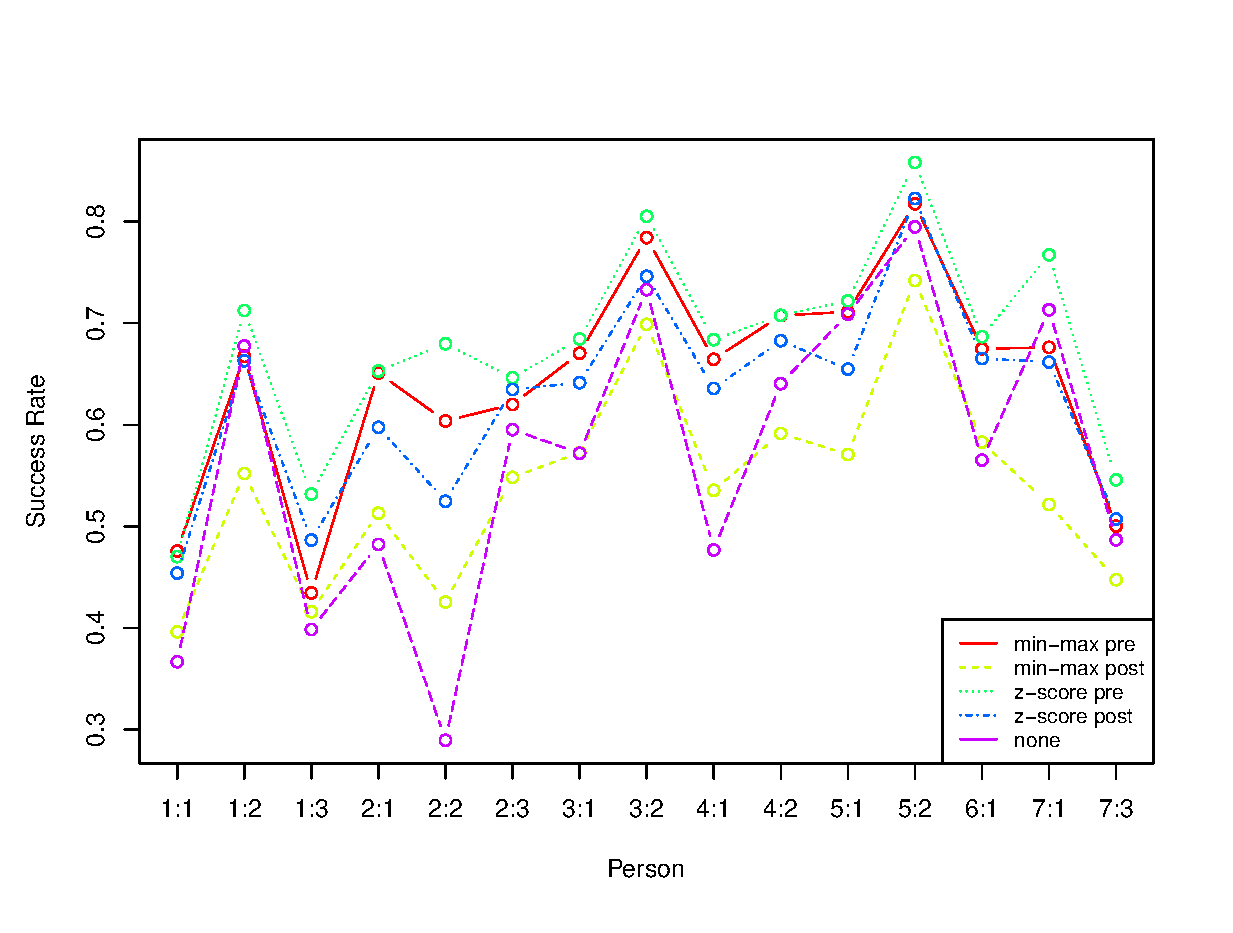
\includegraphics[width = \textwidth]{graphics/graph_normalization}
\caption[Comparison of different students.]{Success rate for detection of characters of on person when not in the training set. 
Data normalized before (pre) and after (post) dataset reduction using PCA.
PCA was set to ensure that 80\% of all variance was included in the data set and K as 10.
The person tested for is given as 'Group':'Member'.
It was tested with 16 people.}
\label{fig:normalization_test_pre-post}
\end{figure}

The mean success rate of figure \ref{fig:normalization_test_pre-post} is listed in table \ref{tab:meanSuccess_normalization_test_pre-post}.
From both the graph and table, it can be concluded that the z-score standardization before the PCA reduction performs, on average, at least 3\% better than the other methods.

The figure \ref{fig:normalization_test_pre-post} also shows that in general all three normalizations, except for the min-max normalization after PCA reduction, is on average, yielding a higher number of correct predictions.

The normalization before the PCA reductions yields a better result in all cases. 
This may be because it enables the PCA to find the features being more responsible for the decision of which category a element belongs to. 
Some of the performance improvement can be because of features of a low variance in their measured value, have a larger relevance as to what the actual category of the elements are.

\textbf{UPDATE TABLE!}

\begin{table}[H]
\centering
\begin{tabular}{|l|r|}\hline
% 0.5720167 0.4639500 0.6055167 0.5521333 0.5034333
Normalization Method & Mean Success \\ \hline
Min-Max Normalization Pre & 57.2 \% \\ \hline
Min-Max Normalization Post & 46.4 \% \\ \hline
Z-Score Normalization Pre & 60.6 \% \\ \hline
Z-Score Normalization Post & 55.2  \% \\ \hline
No Normalization & 50.3 \% \\ \hline
\end{tabular}
\caption{Mean success rates for normalization test as seen in figure \ref{fig:normalization_test_pre-post}.}
\label{tab:meanSuccess_normalization_test_pre-post}
\end{table}



\subsubsection{Performance Effect when adding a Filter}

\begin{figure}[H]
\centering
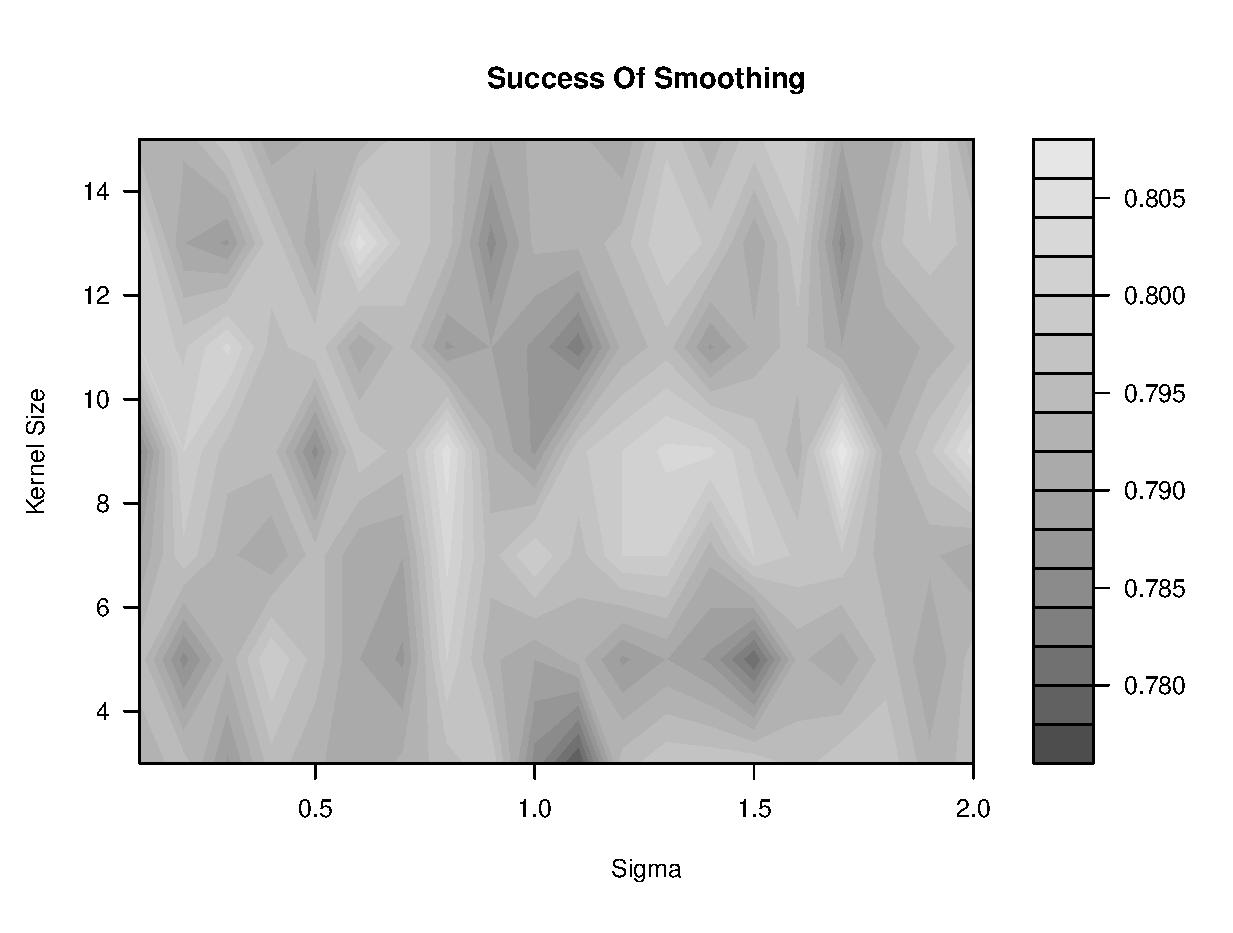
\includegraphics[width = \textwidth]{graphics/success_of_smoothing_contour}
\caption[Optimal smoothing]{Impact of sigma and kernel size when smoothing an image. 
Tested with group 3 member 2's data against 14 other students.
}
\label{fig:smoothing_contour}
\end{figure}

To find the optimal kernel size the success detection rate was plotted with a varying $\sigma$. 
The optimal kernel size is chosen to be 9 pixels wide.
From figure \ref{fig:smoothing_contour} it is concluded that a filter size of 9 is optimal.

Using this knowledge figure \ref{fig:normalization_test_with_smooth} was generated.
The figure compares the unprocessed success rate compared to that of the z-score pre and z-score pre with gaussian smoothing (filter size 9 and sigma 0.7).

 \begin{figure}[H]
 \centering
 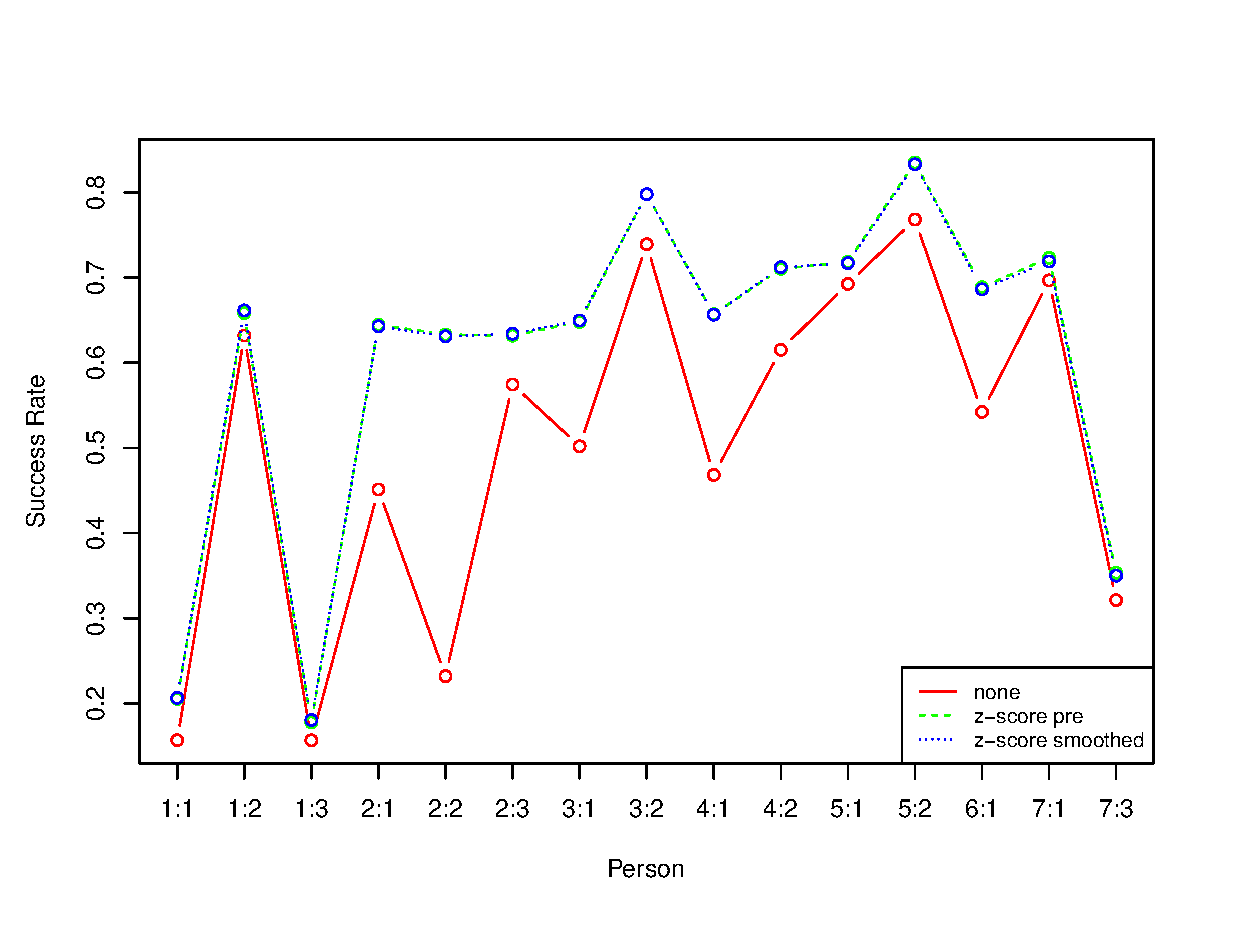
\includegraphics[width = \textwidth]{graphics/graph_normalization_smoothed}
 \caption[Filtered and normalized data.]{Filtered data normalized vs unfiltered normalized data.
 Running each person against the rest of the class in the train set.
 }
 \label{fig:normalization_test_with_smooth}
 \end{figure}

As seen on figure \ref{fig:normalization_test_with_smooth}, then the result of smoothing the data before normalization is not improving the data.


\input{sections/bayes/preprocessing}

\subsection{Naive Bayes Optimization}

The timing was measured with different bin sizes. 
In figure \ref{fig:baye_timing} the timing and success can be seen.
The timing is linear and there is no increase in successful classifications with more than 100 bins. 
The time it took to normalize the data into bins and calculate the naive Bayes is shown.

\begin{figure}[H]
\centering
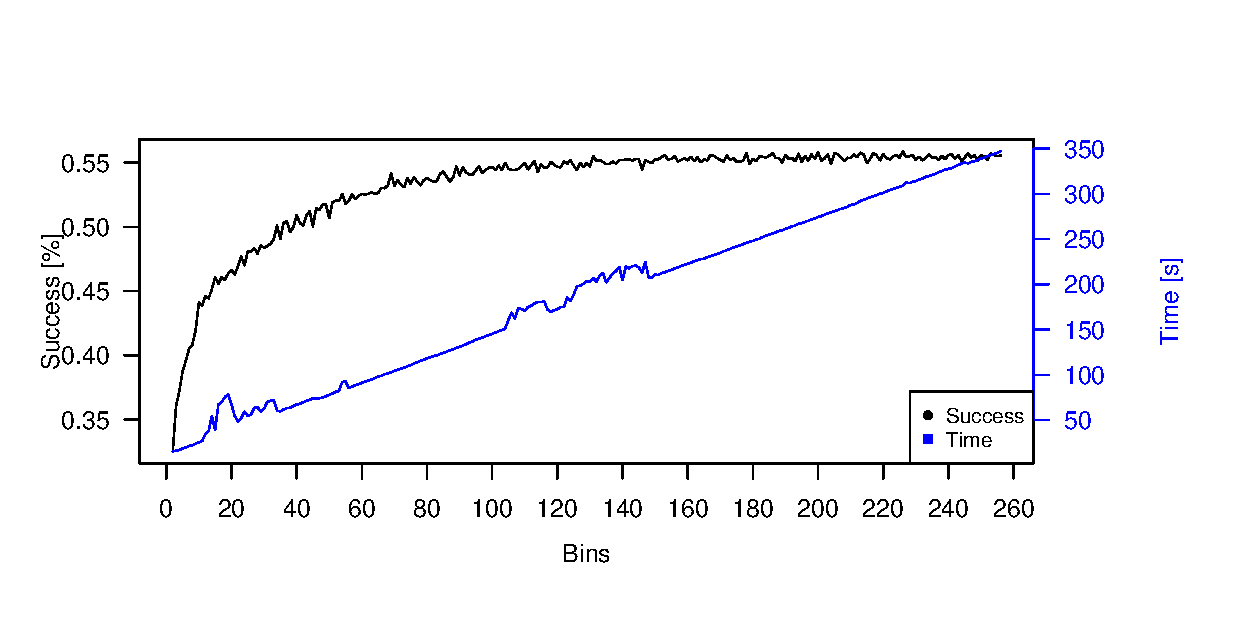
\includegraphics[width = \textwidth]{graphics/baye_timing_bins}
\caption[Timing with different bin sizes]{Timing and success of different bin sizes. Data was tested on Group 3 member 2's data vs 16 people.}
\label{fig:baye_timing}
\end{figure}


The best values for bins and PCA are taken from figure \ref{fig:contour_bin-vs-pca} and then used to compare every person with the rest of the class as seen in figure \ref{fig:comp_naiveBayes}.

\begin{figure}[H]
\centering
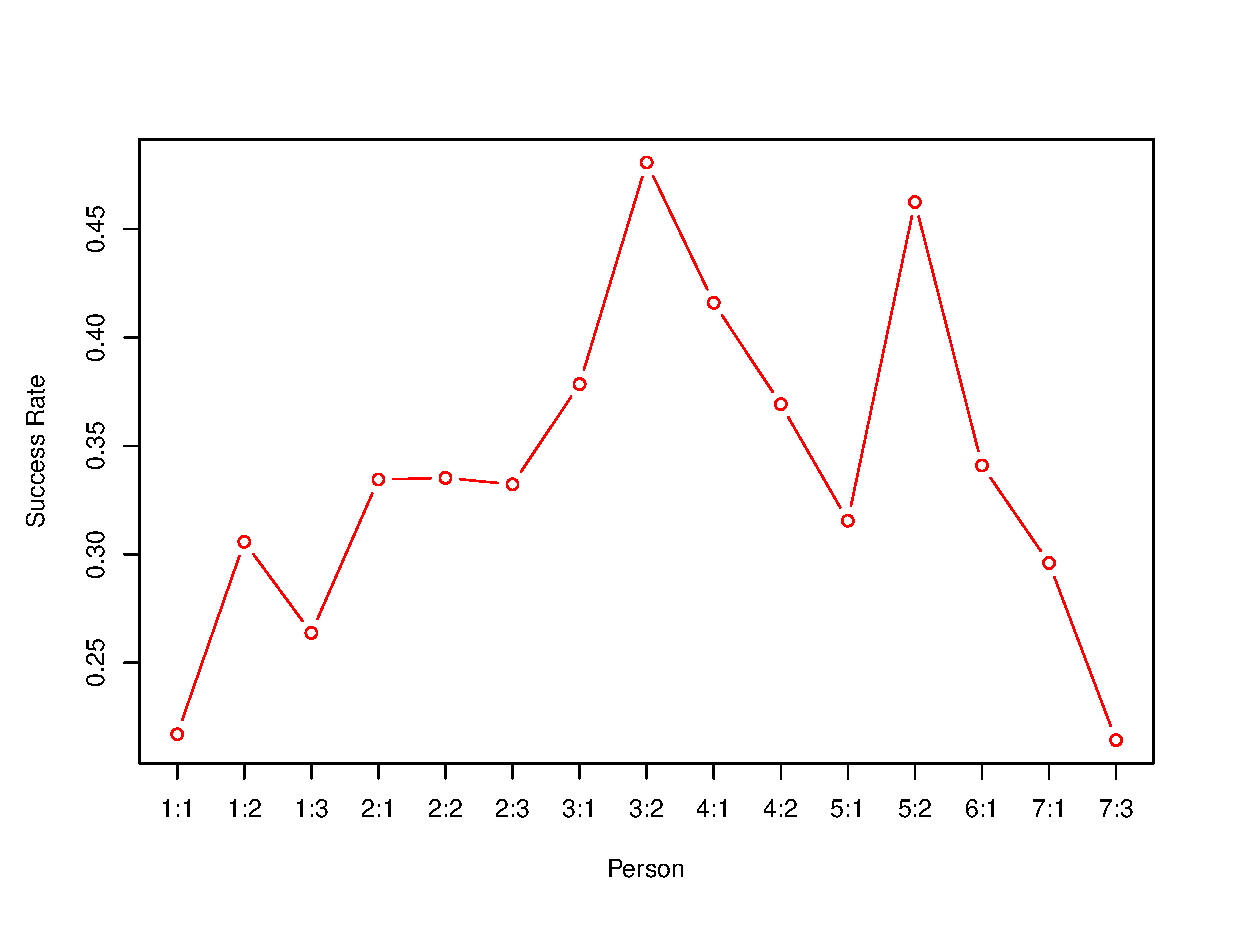
\includegraphics[width = \textwidth]{graphics/graph_baye_comparison}
\caption{Comparison of Naive Bayes for one person with the rest of the class.
Where bins is 50 and PCA is 50\%. The mean success rate is 34.6\%.}
\label{fig:comp_naiveBayes}
\end{figure}

From here it can be seen that this method performs rather bad when testing on the whole class.
With a mean success of 34.6\% for the Naive Bayes, the chance of detecting a decimal correctly is considerably worse than any other previous method  encountered and hence not recommended.

A confusion matrix is also given in table \ref{tb:confus_bayes}.
This is made under same circumstances as figure \ref{fig:comp_naiveBayes} with the test person set to G3M2.

\begin{table}[H]
\centering
	\begin{subtable}{0.75\textwidth}
        \centering
        
\begin{tikzpicture}
            \node at (0,0) {\Large Actual Class}; 
        \end{tikzpicture}
    \end{subtable}
    
    \begin{subtable}{0.05\textwidth}
        \flushright
        
\begin{tikzpicture}
            \node[rotate=90] {\Large Predicted Class};
        \end{tikzpicture}
    \end{subtable}
    \begin{subtable}{0.7\textwidth}
            \centering
%            {\scriptsize
                \begin{tabular}{l|*{10}{c}}
                    &0	& 1	& 2	& 3	& 4	& 5	& 6	& 7	& 8	& 9 \\
\hline
0	& 311	& 8	& 17	& 0	& 1	& 57	& 15	& 13	& 4	& 4 \\
1	& 13	& 247	& 58	& 19	& 19	& 17	& 9	& 37	& 33	& 41 \\
2	& 7	& 5	& 116	& 8	& 0	& 5	& 14	& 32	& 33	& 0 \\
3	& 2	& 18	& 3	& 106	& 0	& 2	& 11	& 50	& 22	& 3 \\
4	& 15	& 15	& 12	& 26	& 323	& 37	& 47	& 92	& 3	& 73 \\
5	& 8	& 4	& 3	& 16	& 0	& 81	& 2	& 0	& 10	& 10 \\
6	& 12	& 38	& 76	& 42	& 5	& 98	& 260	& 5	& 39	& 9 \\
7	& 0	& 1	& 1	& 2	& 0	& 10	& 0	& 109	& 1	& 0 \\
8	& 25	& 45	& 111	& 150	& 0	& 59	& 27	& 15	& 218	& 11 \\
9	& 7	& 19	& 3	& 31	& 52	& 34	& 15	& 47	& 37	& 249 \\

                \end{tabular}
%            }
    \end{subtable}
    \caption{Confusion matrix for Naive Bayes.
    Where bins is 50 and PCA is 50\%. The total success is 50.5\%.}
    \label{tb:confus_bayes}
\end{table}

The data from the confusion matrix in table \ref{tb:confus_bayes} is used to group the ten different decimals into three different groups depending on how well they are detected.
These are seen in table \ref{tab:dec_eval_confus}.

\begin{table}[H]
\centering
\begin{tabular}{|l|c|}
\hline
Group & Decimal \\ \hline
Good ($\geq$ 75\%) & 0, 4 \\ \hline
Intermediate (50\% to 75\%) & 1, 6, 8, 9 \\ \hline
Bad ($\leq$ 50\%) & 2, 3, 5, 7 \\ \hline
\end{tabular}
\caption{Decimal evaluation of confusion matrix in table \ref{tb:confus_bayes}.}
\label{tab:dec_eval_confus}
\end{table}

As can be seen in table \ref{tab:dec_eval_confus}, then the detection of 0 and 4 is quite good, but there is a large amount of miss detected numbers.
The 2's and 3's are often confused with the 8 and the 5 is in many cases confused with the 6.
It can furthermore be seen that the classes 5 and 7 are rarely used to describe a prediction.
Why this is so could be due to their close resemblance to the other classes such as 6 in the case of 5.



\end{document}